
\begin{figure}[h]
\centering
\begin{subfigure}[b]{0.5\textwidth}\centering
\resizebox{0.8\linewidth}{!}{%
\begin{tikzpicture}[
  every node/.style={align=center, font=\scriptsize},
  level 1/.style={sibling distance=26mm, level distance=9mm},
  level 2/.style={sibling distance=30mm, level distance=11mm},
  level 3/.style={sibling distance=15mm, level distance=11mm},
  level 4/.style={sibling distance=15mm, level distance=11mm},
  edge from parent/.style={draw,-}
]
\node {$N_0:\{\mathrm{AG}\,\mu\wedge\mathrm{AG}(q\!\rightarrow\!\sigma)\}\ \ANDn$}
 child { node {$N_1:\{\,\}$\\ $\OPEN$}
   edge from parent node[left,font=\tiny,pos=.45]{\rl{discharge}} }
 child { node {$N_2:\{\mu^{\ast},\neg q\vee\sigma\},\ x{:=}0$\\ $\Deadline{=}\{x\le 4\}\ \ORn$}
   child { node {$N_3:\{\neg q,\mu^{\ast}\}\ \ORn$}
     child { node {$\CLOSED$\\ $q\wedge\neg q$}
       edge from parent node[left,font=\tiny,pos=.45]{\rl{Ustopcarry}} }
     child { node {$\CLOSED$\\ $\rl{Ugocarry}$\\ needs $x>4$}
       edge from parent node[right,font=\tiny,pos=.45]{\rl{Ugocarry}} }
     edge from parent node[left,font=\tiny,pos=.45]{$\neg q$} }
  child { node {$N_4:\{q,\mu^{\ast},\sigma^\bullet\}$\\ $x{:=}0,\ z{:=}0,\ \Deadline{=}\{x\le3\}$}
     child { node {$N_5:\{\neg q,\mu^{\ast},\sigma^\bullet\}$\\ $x{=}z\in(0,3]\ \ORn$}
       child { node {$\CLOSED$\\ \rl{Ustopcarry} \\needs $q$}
         edge from parent node[left,font=\tiny,pos=.45]{\rl{Ustopcarry}} }
       child { node {$\CLOSED$\\ \rl{Ugocarry} \\needs $x>3$}
         edge from parent node[right,font=\tiny,pos=.45]{\rl{Ugocarry}} }
       edge from parent node[right,font=\tiny,pos=.45]{\rl{Delay}, \rl{EX}} }
     edge from parent node[right,font=\tiny,pos=.4]{$\sigma$; \rl{launch}, \rl{Ustopcarry}} }
   edge from parent node[right,font=\tiny,pos=.45]{$(\wedge)$, \rl{launch}, \rl{Carry}} };
\end{tikzpicture}}
\subcaption{$\mathrm{AG}(\mathrm{AF}_{[1,4]} q)\wedge\mathrm{AG}(q \rightarrow
\mathrm{AG}_{(0,3]}(\lnot q))$.}
\label{fig:ex-roll}
\end{subfigure}
\hfill
\begin{subfigure}[b]{0.48\textwidth}\centering
\resizebox{0.9\linewidth}{!}{%
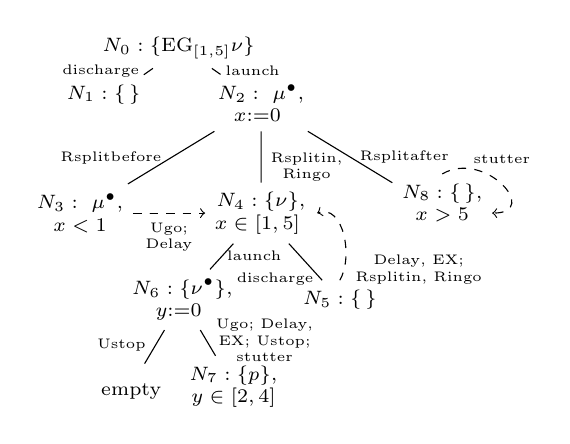
\begin{tikzpicture}[
  every node/.style={align=center, font=\scriptsize},
  level 1/.style={sibling distance=20mm, level distance=7mm},
  level 2/.style={sibling distance=23mm, level distance=14mm},
  level 3/.style={sibling distance=20mm, level distance=11mm},
  level 4/.style={sibling distance=13mm,level distance=11mm},
  edge from parent/.style={draw,-}
]
\node {$N_0:\{\mathrm{EG}_{[1,5]}\nu\}\ \ANDn$}
 child { node {$N_1:\{\,\}$\\ $\OPEN$}
   edge from parent node[left,font=\tiny,pos=.45]{\rl{discharge}} }
 child { node {$N_2:\ \mu^\bullet,$\\$x{:=}0\ \ANDn$}
   child { node (bef) {$N_3:\ \mu^\bullet,$\\$ x<1$}
    edge from parent node[left,font=\tiny,pos=.5]{\rl{Rsplitbefore}} }
   child { node (in) {$N_4:\{\nu\},$\\$ x\in[1,5]\ \ANDn$}
     child { node {$N_6:\{\nu^\bullet\},$\\$ y{:=}0\ \ORn$}
       child { node {$\CLOSED$\\ empty}
         edge from parent node[left,font=\tiny,pos=.45]{\rl{Ustop}} }
       child { node {$N_7:\{p\},$\\$ y\in[2,4]$}
         edge from parent node[right,font=\tiny,pos=.4]{\rl{Ugo}; \rl{Delay},\\ \rl{EX}; \rl{Ustop}; \\stutter} }
       edge from parent node[right,,xshift=-2pt,font=\tiny,pos=.45]{\rl{launch}} }
       child { node (disch) {$N_5:\{\,\}$}
       edge from parent node[left, yshift=-7pt,xshift=7pt,font=\tiny,pos=.45]{\rl{discharge}} }
     edge from parent node[right,font=\tiny,pos=.7]{\rl{Rsplitin},\\ \rl{Ringo}} }
   child { node (aft) {$N_8:\{\,\},$\\$ x>5$\\ $\OPEN$}
     edge from parent node[right,font=\tiny,pos=.5]{\rl{Rsplitafter}} }
   edge from parent node[right,font=\tiny,pos=.45]{\rl{launch}} };
\draw[->,dashed] (bef.east) to[out=0,in=180,looseness=.7]
  node[below,font=\tiny,pos=.5]{\rl{Ugo}; \\\rl{Delay}} (in.west);
\draw[->,dashed] (disch.north) to[out=60,in=20,looseness=1]
  node[right,yshift=-4pt,font=\tiny,pos=.25]{\rl{Delay}, \rl{EX};\\ \rl{Rsplitin}, \rl{Ringo} } (in.east);



\draw[->,dashed] (aft.north) to[out=30,in=0,looseness=2]
  node[above, yshift=4pt,font=\tiny]{stutter} (aft.east);
\end{tikzpicture}}
\subcaption{$\mathrm{EG}_{[1,5]}\tEU{\top}{p}{[2,4]}$.}\label{fig:ex-zeno}
\end{subfigure}
\caption{Two tableau runs. %$\ANDn$ marks an AND-node;$\ORn$ an OR-node. 
$\OPEN$ marks an open node, $\CLOSED$ a closed
one.}\label{fig:ex2}
\end{figure}